\documentclass{article}
%\usepackage{arxiv}
\usepackage[numbers,sort&compress,super,comma]{natbib} % this must be before neurips_2024
\usepackage[preprint]{neurips_2025}
\usepackage[utf8]{inputenc}
\usepackage[english]{babel}
\usepackage{amssymb, amsmath, amsthm, amsfonts}
\usepackage{thmtools, mathtools, mathrsfs, dsfont}
\usepackage{bbm}
%\usepackage{bbold} %for mathbb{1}
\usepackage{forloop}
\usepackage[pdftex]{graphicx}  %remove demo option in your document
\usepackage{sidecap}
\usepackage{enumerate}
\usepackage[shortlabels]{enumitem} %easy customization of itemize/enumerate lists
\PassOptionsToPackage{dvipsnames}{xcolor}
\usepackage{xcolor}
\definecolor{ForestGreen}{rgb}{0.13, 0.55, 0.13}
\definecolor{MidnightBlue}{rgb}{0.1, 0.1, 0.44}
\definecolor{BurntOrange}{rgb}{0.8, 0.33, 0.0}
\definecolor{Plum}{rgb}{0.56, 0.27, 0.52}
\usepackage[colorlinks=true,linkcolor=MidnightBlue,citecolor=ForestGreen,filecolor=TealBlue,urlcolor=Plum]{hyperref}
\hypersetup{breaklinks=true}
\usepackage{tikz}
\usetikzlibrary{positioning}
\usepackage{tikz-cd}


%for comments
\newcommand{\ptitle}[1]{\textbf{#1:}\xspace}
\definecolor{mpcolor}{rgb}{1, 0.1, 0.59}
\definecolor{ascolor}{rgb}{1, 0.5, 0.}
\newcommand{\mpcomment}[1]{\textcolor{mpcolor}{(#1)}}
\newcommand{\ascomment}[1]{\textcolor{ascolor}{(#1)}}

\graphicspath{{figures}}

\newtheorem{theorem}{Theorem}
\newtheorem{proposition}{Proposition}
\newtheorem{lemma}{Lemma}
\newtheorem{corollary}{Corollary}[theorem]
\theoremstyle{definition} \newtheorem{definition}{Definition}  \newtheorem{example}{Example}
\theoremstyle{remark} \newtheorem{remark}{Remark}


\newcommand{\reals}{\mathbb{R}}
\newcommand{\sep}{\operatorname{sep}}
\newcommand{\cl}{\operatorname{cl}}
\newcommand{\vol}{\operatorname{vol}}
\newcommand{\boa}{\operatorname{BoA}}
\newcommand{\mcN}{\mathcal{N}}
\newcommand{\mcK}{\mathcal{K}}
\newcommand{\mcU}{\mathcal{U}}
\newcommand{\mcX}{\mathcal{X}}
\newcommand{\T}{\operatorname{T}}
\newcommand{\TR}{\T\!\mathbb{R}}
\newcommand{\TM}{\T\!M}
\newcommand{\TpM}{\T_p\!M}
\newcommand{\Diff}{\operatorname{Diff}}
\newcommand{\Hpert}{H^{\text{pert}}}
\newcommand{\inv}{\operatorname{Inv}}
\newcommand{\manifold}{\mathcal{M}}

\newcommand{\defvec}[1]{\expandafter\newcommand\csname v#1\endcsname{{\mathbf{#1}}}}
\newcommand{\dm}[1]{\ensuremath{\mathrm{d}{#1}}} % dx dy dz dmu
\newcounter{ct}
\forLoop{1}{26}{ct}{
    \edef\letter{\alph{ct}}
    \expandafter\defvec\letter
}

% captial \vA
\forLoop{1}{26}{ct}{
    \edef\letter{\Alph{ct}}
    \expandafter\defvec\letter
}


%\title{Interpretable attractor motifs for a new language for neural computation}
\title{Attractor motifs for an interpretable language for working memory-type neural computation}
%Dynamical Motif Extraction for Interpretable Neural Computation
% Interpretable Neural Computation via Dynamical Motifs
\author{\'Abel S\'agodi and Il Memming Park}
\date{\today}



\begin{document}
\maketitle

% keywords: interpretability; similarity metric; neural computation; working memory; computation through dynamics

\section*{Abstract}

Understanding computation in dynamical neural systems often requires interpreting the behavior of large, black-box models.
This poses challenges for both interpretability and cross-model comparison—particularly when comparing models from different sources, such as two animals.
To address this, we propose a framework for interpreting neural computation in working memory through \emph{dynamical motifs}—canonical, human-understandable building blocks of dynamics.
Within this framework, we introduce a model reduction method that approximates the essential computational mechanism in a neural system by identifying small perturbations that render two systems topologically conjugate.
This allows us to define and quantify similarity between systems in terms of shared dynamical structure.
The extracted motifs are robust to architectural and parametric variation, suggesting they reflect stable computational strategies rather than model idiosyncrasies.
Our method uses a curated library of low-dimensional canonical motifs (e.g., limit cycles, ring attractors, bounded line attractors) to explain the core dynamics.
We demonstrate the approach by extracting a ring attractor motif from a high-dimensional RNN trained on a delayed match-to-sample task, and show how the motif captures the essential geometry and dynamics underlying working memory.
Our results highlight the utility of this method for robust interpretation and cross-system comparison within the computation-through-dynamics paradigm.


\section{Introduction}\label{sec:intro}
Understanding the relationship between neural activity and behavior is a fundamental question in neuroscience.
 Recent research has demonstrated that despite the complexity of neuronal networks, their activity often resides in a low-dimensional manifold, capturing only a fraction of the potential complexity of the system \citep{duncker2021dynamics}.
 This observation suggests that neural activity is shaped by strong underlying constraints, possibly imposed by behaviorally relevant computations and external environmental demands.

Behavior, in many cases, is surprisingly simple. Even in seemingly complex tasks, animals and humans exhibit structured, stereotyped actions that can often be described using a small number of latent variables. From motor control to decision-making, behavioral trajectories unfold in a manner that is both predictable and constrained, hinting at a fundamental simplicity underlying observed actions.
If neural activity is the substrate that generates behavior, then it is natural to expect that it too is organized around similarly low-dimensional, structured dynamics. This assumption motivates the search for interpretable motifs in neural dynamics that mirror the simplicity and regularity of behavior.

If neural dynamics are indeed tuned to drive behavior, we should expect a correspondence between the low-dimensional structure of neural activity and the inherent simplicity of behavior.
 This suggests that much of the apparent complexity in neural recordings may stem from redundant or task-irrelevant variability rather than meaningful high-dimensional computation.
  In this work, we explore the hypothesis that neural representations of behavior are fundamentally simple, reflecting a constrained, low-dimensional organization that enables efficient motor control, decision-making, and cognitive processing.
 Through computational modeling and empirical analyses, we demonstrate how low-dimensional neural manifolds can emerge and how their structure aligns with behavioral simplicity, providing insights into the fundamental principles governing neural computation.
 
 
 
 %big datas
\paragraph{Large datasets}
 As the number of simultaneously recorded neurons increases and experimental paradigms become more complex (e.g. freely behaving animals), it becomes increasingly challenging to develop computational models that can describe the population activity while still providing a meaningful interpretation of how it relates to system-level function.


%multi
\paragraph{Multi-X datasets}
Multiple animals \citep{depasquale2021accumulation}

Multiple tasks \citep{}

\subsection{Our contribution}\label{sec:contribution}
\begin{itemize}
\item we propose a formalism for interpretability for the purpose of identifying neural computations in models of neural dynamics;
\item we propose a way to measure the loss of details in the process of abstraction/reduction to achieve more interpretable models;
\item 
\end{itemize}





\section{Background and related work}\label{sec:background}
A theory of (neural) computation\citep{jaeger2021theory, jaeger2023timescales, jaeger2023theory}
- Dynamical system theory as the source for the syntax for the language of neural computation.
\citep{elgazzar2024universal}

Similar idea: DYNAMO \citep{cotler2023analyzing}

a language describing the axes of the space of possible dynamical solutions and their characteristics \citep{pagan2022dm}

\subsection{Computation through dynamics}
\citep{mante2013context}
\citep{sussillo2014neural}
\citep{vyas2020ctd}
\citep{versteeg2023expressive, sedler2023expressive}
\citep{dinc2025latentcomputing}

latent state space modeling \citep{zoltowski2020general} 
XFADS\citep{Dowling2024b}

Neural Latents Benchmark \citep{pei2neural}
CtD benchmark \citep{versteeg2025computation}

RNNs for neural computation \citep{chaisangmongkon2017transience}
Black box \citep{sussillo2013blackbox}
Reverse-engineering \citep{maheswaranathan2019reverse} \citep{golub2018fixedpointfinder} \citep{smith2021reverse} \citep{rivkind2017local}
Diversity of solutions \citep{maheswaranathan2019universality}\citep{jarne2023initialization} \citep{turner2021charting} \citep{nayebi2021heterogeneity} \citep{zhong2023mechanistic}

engineering neural computation \citep{eliasmith2003neuralengineering, eliasmith2005unified, eliasmith2010describe} \citep{beiran2023rnns}
Engineering RNNs that embody latent task dynamics (EMPJ) \citep{pollock2020engineering}

%\subsubsection{Theoretical neuroscience}
%\citep{thompson2021explanation}
%\citep{levenstein2023theory}

\subsubsection{Examples of neural computation}
\paragraph{Working memory}
Discrete 

Continuous \citep{hoeller2024bridging} \citep{zhang2022translation}

\paragraph{Decision making}

\paragraph{Motor control}
\citep{wang2022representation}

\subsubsection{Canonical models for neural computation}
\citep{chirimuuta2014minimal}

Variability in implementation



\subsection{Existing methods for characterizing dynamics}

\begin{figure}[htbp]
    \centering
    \includegraphics[width=0.75\linewidth]{ds_landscape_carving}
    \caption{Caption}
    \label{fig:ds_landscape_carving}
\end{figure}

\subsubsection{Reconstructing dynamics}
Learning interpretable continuous-time models of latent stochastic dynamical systems \citep{duncker2019learning}

Phase2vec \citep{ricci2022phase2vec}
\citep{moriel2024timewarpattend}
Smooth Prototype Equivalences \citep{friedman2025characterizing}

MARBLE \citep{gosztolai2025marble}


\subsubsection{Methods to compare/classify dynamics}\label{sec:compare}
%Comparison of dynamical systems
Concepts:
\begin{itemize}
\item equivalence of systems: topological conjugacy (Def.~\ref{def:top_conj}).%/equivalence
\item asymptotic behavior: $\omega$-limit sets
\end{itemize}

Taking apart topological conjugacy (diffeomorphism from motif):
\begin{itemize}
\item On asymptotic / $\omega$-limit set / invariant set
\item On transients \citep{koch2024biological}
\end{itemize}


DS/RNN analysis
Dyn Sys: Linking parameters and behavior: bifurcation, asymptotic behavior, topological equivalence \citep{beer1995ctrnn, beer2006parameterspace}

For task-trained neural networks
\citep{huang2024measuring}

Bisimilarity\citep{vanderschaft2004bisimulation, vanderschaft2004equivalence, pola2004bisimulation, pola2006equivalence, tabuada2004bisimilar}
approximate bisim\citep{girard2011approximate}

\paragraph{SOTA}
\citep{mezic2004comparison}

assess the limit sets
Fixed-point based \citep{sussillo2013blackbox,katz2017fibers,golub2018fixedpointfinder}

Also limit cycles 
LCs in RNNs \citep{townley2000existence} \citep{pals2024inferring}

slow invariant manifolds\citep{Sagodi2024a}

TWA\citep{moriel2024timewarpattend}

SVCCA\citep{raghu2017svcca}

Dynamical Similarity Analysis (DSA) \citep{ostrow2024beyond} \citep{kamiya2024koopman}\\
What we lose (because of the truncation): limit cycles, multistability
But we can capture some slow manifold behavior!

\citep{libedinsky2023comparing}
\citep{lipshutz2024disentangling} 
\citep{nejatbakhsh2024comparing} Optimal transport
\citep{barbosa2025quantifying}

Diffeomorphic vector field alignment for comparing dynamics across learned models\citep{chen2024dform}
- orbital similarity loss (Eq.~5)



\subsubsection{Decomposition of the dynamics}\label{sec:decomposition}
into basins of attraction through Conley’s Fundamental Theorem for Dynamical Systems \citep{conley1978morse, norton1995fundamental,mischaikow1999cit}

FSM-based approaches\citep{pollack1991induction, casey1996dynamics, jacobsson2005ruleextraction, ashwin2021excitable, oliva2019fsm, cotteret2024fsm}
Behaviorism is based on an engineering approach, treating the mind as a control system for the organism. This corresponds to an approximation of the recurrent neural dynamics (brain states) by finite state automata (behavioral states). Another approximations to neural dynamics is described, leading to a Platonic-like model of mind based on psychological spaces. \citep{duch1998platonic}

neural automata\citep{goles2013neural, uria2024invariants}

For different type of dynamcis (ergodic) but that separates the state space into coherent/metastable regions between which the Perron–Frobenius operator describes transitions.

Main shortcoming: difficulty with dealing with complicated attractors.
When is decomposition of attractor into motifs possible?

On the lifting and reconstruction of nonlinear systems with multiple invariant sets \citep{pan2024lifting}

\citep{driscoll2024flexible}

compositional tasks \citep{tafazoli2024building}

decomposition through population-based modeling\citep{glaser2020recurrent} 

\citep{mudrik2024decomposed}

\paragraph{Neural ensembles}
\citep{yuste2024ensembles}



\subsubsection{Reduction}\label{sec:reduction} %simplification of dynamics
In each basin of attraction we have one attractor.
We can simplify it's dynamics by looking at its normal form.

\begin{itemize}
\item approximation based (model order reduction): \citep{schilders2008model}
\item topology based Delay Embedding and Takens' Theorem  and Morse Decomposition 
\item low-dimensional reduced model \citep{zemlianova2024dynamical} \citep{nonnenmacher2017extracting}
\item motifs: normal forms \citep{full1999templates} \citep{nayfeh2011normalforms} and \citep{bonilla2012discriminative} (also referred to as prototypes in literature)
\item Koopman  Spectral properties of dynamical systems, model reduction and decompositions \citep{mezic2005spectral}, Dynamic Mode Decomposition\citep{rowley2009spectral}, EDMD \citep{mezic2005spectral}
\item \citep{rowley2017model}
\item libraries \citep{brunton2014compressive}, SINDy  one starts with a large library of candidate functions (or dynamical motifs) that could potentially describe the dynamics of a system. The method then uses sparse regression techniques to select a few terms that best capture the observed time-series data \citep{brunton2016discovering, brunton2016sparse, fasel2022ensemble}
\item  primitives: linear \citep{kaul2020linear} (more for behavioral \citep{ijspeert2013dynamical})
\item fast-slow \citep{jones1995gspt} \citep{verhulst2006methods}  \citep{dsilva2016data} \citep{haller2017exact}
\item averaging methods \citep{sanders2007averaging} (invariant tori\citep{novaes2024invariant}), Theorem 9.4 in \citep{hoppensteadt2012weakly}
\item FSMs: \citep{giles1991extracting, casey1996dynamics, giles1999equivalence, oliva2019fsm, ceni2020excitable, cotteret2024fsm, aichernig2024learning} + weighted\citep{wei2024weighted}
\item effective dynamics \citep{menier2025interpretable}
\item Reduction of Limit-Cycle Oscillators to Phase–Amplitude and Phase Models \citep{ashwin2016mathematical} (def. limit-cycle oscillator: attracting and hyperbolic periodic orbit, reduction: reduce per orb. to a description that involves a phase that lives on a topological circle that can be thought of as an interval)
%and T −  are close for  small
%define a phase θ modulo T, 
\item contractivity \citep{lohmiller1998contraction}\citep{bullo2023contraction} \citep{revay2020contracting} \citep{tsukamoto2021contraction} \citep{davydov2022rnn, davydov2024noneuclidean}
\item \citep{li2021novel}
\item \citep{otto2023learning}
\item vector fields projected onto the manifold \citep{roy2021extracting, luo2023noncanonical}
\item spectral submanifold \citep{cenedese2022data, axaas2023fast, bettini2024model, kaszas2024data}
\item surrogate dynamical systems (any citations?)
\end{itemize}



\paragraph{Reduction of dynamics to extract computation}
Formalize through input-output functional.

The \emph{transfer functional} \( \mathcal{T}_f \) maps an input signal \( u(\cdot) \) to an output signal \( y(\cdot) \), possibly given an initial condition \( x_0 \):
\[
\mathcal{T}_f[u](t) = h(x(t)),
\]
where \( x(t) \) is the solution of the initial value problem:
\[
\dot{x}(t) = f(x(t), u(t)), \quad x(0) = x_0.
\]

What is the distance between $\mathcal{T}_f(f)$ and $\mathcal{T}_f(\Phi^{-1}(f+p))$?
A natural notion of distance between the transfer functionals is
\[
\|\mathcal{T}_f - \mathcal{T}_{\Phi^{-1}(f+p)}\| 
:= \sup_{u \in \mathcal{U}} \sup_{t \in [0, T]} 
\left\| \mathcal{T}_f[u](t) - \mathcal{T}_{\Phi^{-1}(f+p)}[u](t) \right\|,
\]
where \( \mathcal{U} \) is a suitable class of input signals (e.g., all inputs with bounded \( L^\infty \)-norm or from a compact set in \( C([0,T], \mathbb{R}^m) \)).

%adjust h to minimize output error of f+p?
find a new readout map $\tilde h$  so that the output error between $f$ and $f+p$ is minimized.


\paragraph{Reduction of dynamics}
Embed attractor of intrinsic dimension $N$ into $\reals^{n+1}$ to be able to map point in the basin of attraction onto representative points on the stable manifold of the attractor motif.

\ascomment{What is simple behavior in terms of the transfer function?}


\subsection{Interpretability}
\ascomment{Should this come before Reduction?}
%phos
What is interpretability? \citep{erasmus2021interpretability}
\citep{madsen2024interpretability}
levels \citep{hochstein2022levels}

%neuro
\citep{whiteway2019interpretable}
\citep{kar2022interpretability}
extrinsic and intrinsic dimensionality\citep{jazayeri2021interpreting}

 machine learning: important yet slippery\citep{lipton2018mythos}	
 Building Blocks of Interpretability \citep{olah2018interpretability}
\citep{beisbart2022interpretability}
simple isn't easy \citep{raz2024ml}
Manipulating and measuring model interpretability\citep{poursabzi2021manipulating}: \ascomment{A way to compare?}
\citep{he2024multilevel}

\subsubsection{Simplicity}
\citep{gao2015simplicity}
\citep{dyer2023simplest}
\citep{quinn2022information}

Canonical realization = the simplest system (in some sense) that produces the same behavior


\paragraph{Visualization}
\citep{deregt2017understanding}
\citep{karpathy2015visualizing}
PHATE \citep{moon2017visualizing}
MPHATE\citep{gigante2019visualizing}
MMPHA\citep{xie2024multiway} 
\citep{madsen2019visualizing}

\subsection{Minimal}
\citep{beer1996toward}
\citep{lafferriere2000minimal}
\citep{chirimuuta2014minimal}
\citep{batterman2014minimal}
\citep{brancazio2023minimal}

\citep{Jordan2019a}

\paragraph{Reduction/idealization/simplification/abstraction}
\citep{marr1976computation, marr2010vision}

\citep{chirimuuta2018mmm} %chirimuuta2022artifacts, chirimuuta2024analogies

\citep{potochnik2021levels,
potochnik2020idealization,
potochnik2017idealization}

\citep{stinson2020idealized}
\citep{chirimuuta2024brain} 

Solomonoff's theory of inductive inference


\subsubsection{Understanding}
\citep{deregt2017understanding}
\citep{potochnik2017idealization}
\citep{guest2023logical}

Understanding brains \citep{marder2015understanding} \citep{lindsay2023testing} \citep{barman2024towards} \citep{dowling2018understanding}
prediction vs understanding \citep{chirimuuta2021prediction}

Understanding information propagation using dynamical systems tools \citep{vogt2022lyapunov}

\paragraph{Explanations: understanding scientific phenomena}
\citep{parascandolo2021learning}

\paragraph{Contextuality and understanding}
What are we interpreting \emph{for}?

Context: Behavior %Computational theory in Marr's levels?
Interpretation in terms of contributions of the transfer functional.


%context: computation %Representation and algorithm in Marr's levels
\paragraph{Understanding computation in terms of dynamics}
Interpretation in terms of a ``compressed'' description of the dynamics.

task's computational demands (e.g., continuous parametrization of memory)



\subsubsection{Works mentioning interpretability}
\citep{whiteway2019interpretable}
\citep{kar2022interpretability}
 Making hippocampal manifolds physiologically interpretable \citep{esparza2023interpretable}
black box to mixture of interpretable models \citep{ghosh2023blackbox}
\citep{schneider2023learnable}
\citep{brenner2024almost}
\citep{menier2025interpretable}
\citep{nonnenmacher2017extracting}

\subsubsection{Our levels of interperetability}
Proposal: guiding principles for a hierarchy of interpretability

1. Message: poset of interpretable models

2. Message: Actions we can perform to reduce complexity
I. introducing hierarchy 
\citep{Vermani2024b}
\citep{geadah2024parsing, geadah2025modeling}
II. decomposition

3. Message: leaving out details for understanding (abstraction), trade-off between interpretability and accuracy


\subsubsection{Interpretability in RNNs}
%static
SVCCA\citep{raghu2017svcca}
dPCA\citep{kobak2016demixed} Principal Component Analysis as a supervised dimensionality reduction method that finds dimensions in population activity space related to experimentally-defined variables, aiding in the interpretation of complex and heterogeneous single-neuron responses

%MinimalRNN\citep{chen2017minimalrnn} more about simplifying gates
Tiny RNN\citep{jian2023tinyrnn}: analysis of the predictive performance of RNNs with varying sizes revealed that merely 1-4 dynamical variables were adequate for an optimal explanation of behavior in reward learning tasks, suggesting that the behavior of animals in these tasks is low-dimensional
model identification of classes of cognitive models\citep{rmus2024artificial}
Towards interpreting recurrent neural networks through probabilistic abstraction \citep{dong2020towards}
Expressive architectures enhance interpretability of dynamics-based neural population models \citep{sedler2023expressive}
Interpretable Latent Factors with Sparse Component Analysis \citep{zimnik2024identifying}
Almost-Linear RNNs Yield Highly Interpretable Symbolic Codes in Dynamical Systems Reconstruction \citep{brenner2024almost}
\citep{he2024multilevel}
\citep{schaeffer2020reverseengineering} Representations and Dynamics Distillations (RADD)
\citep{turner2023simplicity}
FSM: \citep{oliva2019fsm}, \citep{cotteret2024fsm},  ENA \citep{ceni2020interpreting}
low-rank RNNs \citep{beiran2021shaping, valente2022extracting, valente2022probing}
mechanistic \citep{qian2024partial}
\citep{Nassar2018b}

Understanding and controlling the geometry of memory organization in RNNs \citep{haputhanthri2025understanding}

\subsubsection{In neuroscience}
\paragraph{Motor primitives}
In motor cortex, neural trajectories during reaching movements often evolve along a low-dimensional cyclic structure, making it possible to interpret them as dynamical primitives for movement \citep{ijspeert2013dynamical}.

\citep{marton2021efficient}



\subsection{A timescale angle to reduction}
\citep{cavanagh2020diversity}

\section{Matching dynamical motifs}
\subsection{Similarity metric}
Let $f, g\in C^1$ be the vector fields.
Then, there exists a perturbation $p\in C^1$ 
 and a homeomorphism $\Phi:\reals^n\rightarrow\reals^n$ such that 
\begin{equation}\label{eq:}
\|\psi_{f+p} - \Phi(\psi_{g})\|_\infty = 0.
\end{equation}

Therefore, we can define the distance metric $d(f,g) = \inf \|p\|$ with the above constraint.


\subsection{An interpretable motif-centered metric for dynamical systems}\label{sec:aut_motif_metric}
Consider our target dynamical system to be defined on a compact subset of $\reals^n$.

Let $f\in C^1$ define the vector field of our target system
and let $g_i$ be a dynamical motif.
Then, there exists a perturbation $p\in C^1$ 
 and a homeomorphism $\Phi:\reals^n\rightarrow\reals^n$ such that 
\begin{equation}\label{eq:perfect_motif_fit}
\|\psi_{f+p} - \Phi(\psi_{g_i})\|_\infty = 0.
\end{equation}

Therefore, we can define the distance w.r.t. each motif as $d(f,g_i) = \inf \|p\|$ with the above constraint.

Projection of $f$ onto library: we get a vector representing the distances to the motifs in the library.

\ascomment{Convergence during training of RNNs: for task that relies on analog memory to low distance to dynamical motif that is a continuous attractor diffeomorphic to the memory manifold.}



\subsubsection{Recognizable geometric-topological features}
fixed points, limit cycles

continuous attractors

invariant manifolds
manifolds neuro/RNN\citep{langdon2023unifying, can2021emergence,
cueva2021continuous,
gort2024emergence,
mishra2021continual,
chaudhuri2019attractor, ghazizadeh2021slowmanifold, duncker2021dynamics, pezon2024linking}
neuro \citep{fortunato2024nonlinear}

manifold alginment \citep{kuoch2024probing}

approximate continuous attractors as slow invariant manifolds\citep{Sagodi2024a}


\subsection{Motifs: The building blocks}
\subsubsection{Guiding principles}
Attractors reduce behavior to "basins" in phase space

human-compatible descriptions

motifs should be all topologically distinct (not topologically conjugate)

%\subsubsection{The base case} % \subsubsection{Constructing}


\paragraph{Enumerating attractors dimension-wise}
In dynamical systems, attractors can be systematically classified according to their topological dimension, with the simplest topological spaces serving as the fundamental building blocks at each level. This perspective provides a principled way to enumerate attractors that can arise in ordinary differential equations (ODEs).
\begin{enumerate}[start=0,label={\bfseries Dim \arabic*:}]
\item  Stable fixed point
\item  Bounded line attractor ($[0,1]\subset\reals$), ring attractor ($S_0^1$), stable limit cycle ($S_1^1$)
\item Plane attractor ($[0,1]^2$), Cylinder attractor ($[0,1]\times S_0^1$), Cylinder-LC attractor ($[0,1]\times S_1^1$), Torus attractor ($(S_0^1)^2$), Torus-LC attractor ($S_0^1\times S_1^1$), QPTA ($(S_1^1)^2$), Sphere attractor $S^2$
\item ...
\end{enumerate}

This pattern continues, with higher-dimensional attractors constructed from fundamental topological spaces such as $S^n$ or their Cartesian and toroidal products.

\ascomment{do we need to account for the possible existence of an attractor of the form $[0,1]^2\setminus D_{1/2}$? It won't affect the loss! So not for now!}


\paragraph{Manifold decomposition}
Triangulation

\subsection{Dynamical motif matching}
\subsubsection{Single global attractor}
We consider a target dynamical system $\dot{x} = f(x)$ which has a single global attractor.
 We assume that this system is topologically equivalent to one of a family of attractor motifs defined by dynamical systems $\dot{y} = g_i(y)$ where each $g_i$ represents a different canonical attractor in its normal form.
  This means that there exists a homeomorphism $\Phi$ mapping solutions of $g_i$ to solutions of $f$.
  Assuming smoothness, we model $\Phi$ as a diffeomorphism.
Our goal is to determine both the correct (best fitting/most explanatory) attractor motif $g_i$ and the diffeomorphism $\Phi$ given only observed trajectories $\{x_j(t_k)\}$ sampled from $f$.

\paragraph{Trajectory based loss function}
Since we do not have direct access to the vector field but only to sampled trajectories, we approximate the system using a learned diffeomorphism \( \hat{\Phi}_\theta \), parameterized by a normalizing flow\citep{kobyzev2020normalizing,papamakarios2021normalizing}, an invertible ResNet\citep{he2016deep}, or a Neural ODE (NODE) \citep{chen2018neural}.
 We seek to minimize the discrepancy between the transformed trajectory and the corresponding trajectory in one of the candidate motifs.

%time repraram
 If the correct motif \( g_i \) is selected, then there should exist an approximate reparametrization of time \( \tau(t) \) such that
\[
y(\tau(t)) \approx x(t),
\]
where \( y(t) \) is a trajectory obtained by integrating \( \dot{y} = g_i(y) \) from an initial condition \( y(0) \). % (close to y(0))


A loss function capturing this trajectory discrepancy is given by:
\[
\mathcal{L}(\theta, i) = \sum_{t} \Big\| (x(t)) - \hat{\Phi}_\theta^{-1}(y(t)) \Big\|^2,
\]
where \( y_{\text{model}}(t) \) is computed via numerical integration of \( g_i \) from an initial condition inferred from the transformed data.

The final optimization objective is:
\[
\min_{\theta, i} \mathcal{L}(\theta, i). % + \lambda \mathcal{R}(\theta), %regularization? NODE\citep{finlay2020trainnode}
\]
%where \( \lambda \) is a regularization coefficient.

This formulation allows for the joint identification of both the correct attractor motif \( g_i \) and the transformation \( \Phi \) that maps the observed system into its canonical/normal form.


\subsection{Application on simple example}
\begin{figure}[htbp]
    \centering
    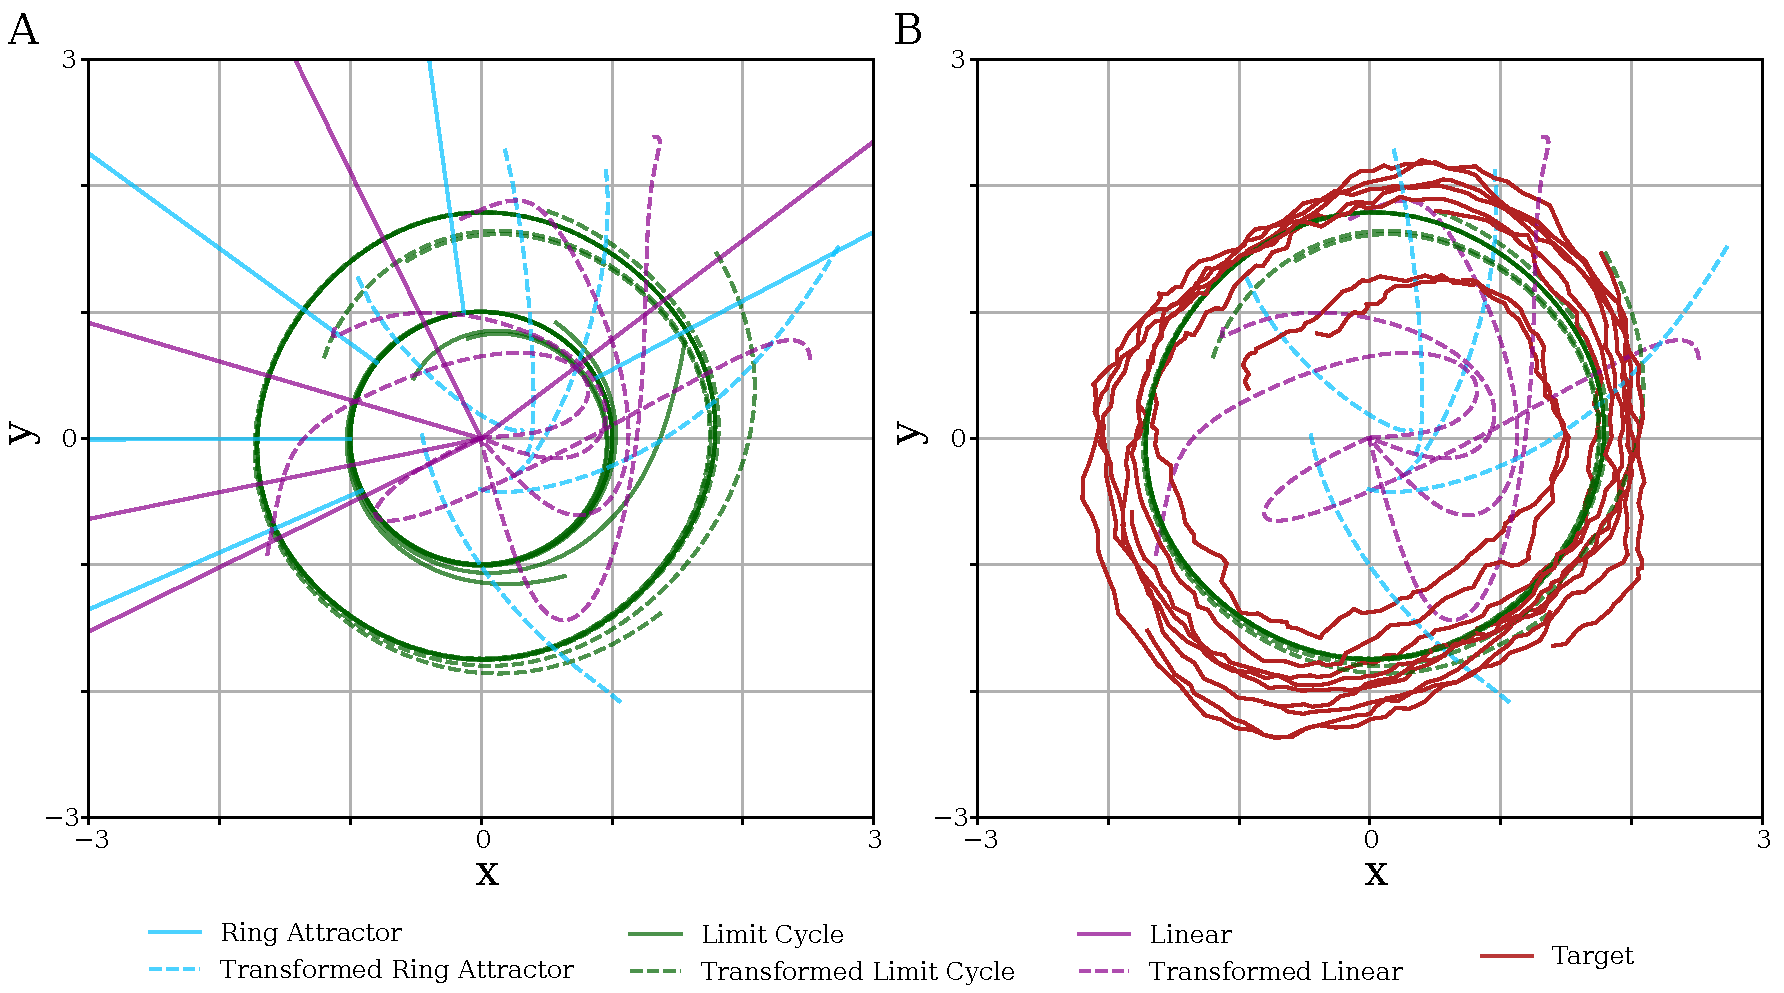
\includegraphics[width=.9\linewidth]{all_motifs_vdp_noisy_var1_ntraj5_ai}
    \caption{Comparison of fitting different motifs to the noisy trajectories generated by a Van der Pol oscillator. The motifs considered in the fitting process include a ring attractor, limit cycle, and fixed point/linear system, sourced from a predefined motif library. The fitting is evaluated based on how well each motif captures the dynamics of the noisy oscillatory data.}
    \label{fig:all_motifs_vdp}
\end{figure}



\subsection{Reducing the dimensionality} % to a minimal dimensional motif
\subsubsection{Homeomorphism from minimal dimensional motif}
Let \( f \in C^1 \) define the vector field of a target dynamical system on \( \mathbb{R}^n \), and let \( g_i \in C^1(\mathbb{R}^m, \mathbb{R}^m) \) be a dynamical motif of minimal dimension \( m \leq n \) that captures the essential dynamics of \( f \). Then there exists a perturbation \( p \in C^1(\mathbb{R}^n, \mathbb{R}^n) \) and a homeomorphism \( \Phi: \mathbb{R}^m \to \mathbb{R}^n \) such that the flow \( \psi_{f+p} \) of the perturbed system is topologically conjugate to the embedded flow \( \Phi \circ \psi_{g_i} \), i.e.,
\begin{equation}\label{eq:hom_from_motif}
\|\psi_{f+p} - \Phi \circ \psi_{g_i} \|_\infty = 0.
\end{equation}


\subsubsection{Surjective mapping to minimal dimensional motif}
Let \( f \in C^1(\mathbb{R}^n, \mathbb{R}^n) \) define the vector field of a target dynamical system, and let \( g_i \in C^1(\mathbb{R}^m, \mathbb{R}^m) \) be a dynamical motif of minimal dimension \( m \leq n \) that captures the essential dynamics of \( f \). Then there exists a perturbation \( p \in C^1(\mathbb{R}^n, \mathbb{R}^n) \) and a surjective continuous map \( \Phi: \mathbb{R}^n \to \mathbb{R}^m \) such that the flow \( \psi_{g_i} \) of the motif is semi-conjugate to the flow \( \psi_{f+p} \) of the perturbed system via \( \Phi \), i.e.,
\begin{equation}\label{eq:perfect_motif_fit}
\| \psi_{g_i} - \Phi \circ \psi_{f+p} \|_\infty = 0.
\end{equation}





\section{Comparison to other methods}



\section{Discussion}

Limits to neuroscientific understanding \citep{chirimuuta2024brain}


simplest isn't always the best \citep{dyer2023simplest}


planning: complex dynamical motifs that correspond to current and future actions \citep{vyas2020ctd}


\newpage
\bibliographystyle{unsrtnat_IMP_v1}
\bibliography{../all_ref.bib,../catniplab.bib}
\newpage
\appendix



%%%%%TOP
\section{Topology}\label{sec:topology}

\subsection{Approximating homeomorphisms}\label{sec:homeomorphisms}


Any homeomorphism on a $p$-dimensional Euclidean space can be approximated by a Neural ODE or an i-ResNet operating on a $2p$-dimensional Euclidean space \citep{zhang2020approximation}.

Capping a Neural ODE or an i-ResNet with a single linear layer is sufficient to turn the model into a universal approximator for non-invertible continuous functions \citep{zhang2020approximation}.

\subsubsection{Implementations}



\subsection{Approximating diffeomorphisms}\label{sec:diffeomorphisms}

a simple sufficient condition for a family of flows on a smooth compact manifold $M$ to generate the group $\Diff0_(M)$ of all diffeomorphisms of M that are isotopic to the identity \citep{caponigro2010families}.

Stability of diffeomorphisms implies that $\Diff(M)\subset C^1(M,M)$  is an open subset.

Normalizing flows\citep{kobyzev2020normalizing}

\paragraph{ResNets}
the layers of a ResNet can be considered as Euler-discretization of the integration of a flow of a diffeomorphism\citep{rousseau2020residual}


\paragraph{Flow-based}
NODE\citep{finlay2020trainnode}
\citep{torchdiffeq}

Conjugate Mappings \citep{bramburger2021conjugate}

%any homeomorphism on a $p$-dimensional Euclidean space can be approximated by a Neural ODE or an i-ResNet operating on a $2p$-dimensional Euclidean space \citep{zhang2020approximation}
Any homeomorphism of $\mathbb {R} ^{n}$ can be approximated by a neural ODE operating on $\mathbb {R} ^{2n+1}$, proved by combining Whitney embedding theorem for manifolds and the universal approximation theorem for neural networks  \citep{zhang2020approximation}

diffeomorphisms from gradient information of desired costs \citep{lai2021parallelised}

\subsubsection{Decomposing diffeomorphisms}\label{sec:diff_dec}
\paragraph{Lie}
Since diffeomorphisms form a Lie group under composition, a diffeomorphism 
\( f \) can be written formally as:
\[
f = \exp(X),
\]
where \( X \) is a vector field (i.e., an element of the Lie algebra of the diffeomorphism group). Expanding \( X \) in a Fourier basis:
\[
X(x) = \sum_k \hat{X}(k) e^{i k \cdot x}
\]
provides a Fourier-like decomposition of the infinitesimal generator.

\subsubsection{Implementations}
Freia\citep{freia} %https://github.com/vislearn/FrEIA

\citep{dinh2016density} % https://github.com/AxelNathanson/pytorch-normalizing-flows?tab=readme-ov-file

\citep{stimper2023normflows} % https://github.com/VincentStimper/normalizing-flows



\newpage
\section{Geometry}
Geometric Learning on Manifolds\citep{mostowsky2024geometrickernels}


\paragraph{Standard Matérn Kernel (Based on Geodesic Distance)}
Replace the Euclidean distance  $\| x - x' \|$  in the Matérn kernel with the distance to the manifold  $ d_{\text{manifold}}(x, x')$. 
This distance is now the measure of how far two points are from each other, but considering the geometry of the manifold.
\begin{equation}
k(x, x') = \frac{1}{\Gamma(\nu)} \left( \frac{\sqrt{2\nu} d_{\text{manifold}}(x, x')}{\ell} \right)^\nu K_\nu\left( \frac{\sqrt{2\nu} d_{\text{manifold}}(x, x')}{\ell} \right).
\end{equation}


\subsection{Implementations}
\citep{miolane2020geomstats}
%https://github.com/geomstats/geomstats?tab=readme-ov-file





%%%%%DS
\newpage
\section{Dynamical systems background}

\subsection{Comparing dynamics}
Binary/Discrete: equivalence

Continuous comparison: metric/distance/dissimilarity



\subsubsection{Exact equivalence: Topological conjugacy}\label{sec:top_conj}

Topological conjugacy is an equivalence relation on the category of flows.
\begin{definition}\label{def:top_conj}
let $\phi$ be a flow on $X$, and $\psi$ a flow on $Y$, with $X$, $Y$, and $h\colon Y \to X$ as above.

We say that $\phi$ is \emph{topologically semiconjugate} to $\psi$ if, by definition, $h$ is a surjection such that
\[
\phi(h(y), t) = h \circ \psi(y, t), \quad \text{for all } y \in Y, \; t \in \mathbb{R}.
\]
Furthermore, $\phi$ and $\psi$ are said to be \emph{topologically conjugate} if they are topologically semiconjugate and $h$ is a homeomorphism.
\end{definition}

Smooth equivalence is an equivalence relation in the category of smooth manifolds with vector fields.
\begin{definition}\label{def:smooth_equivalence}
Two dynamical systems defined by the differential equations 
\[
\dot{x} = f(x) \quad \text{and} \quad \dot{y} = g(y)
\]
are said to be \emph{smoothly equivalent} if there exists a diffeomorphism \( h \colon X \to Y \) such that
\[
f(x) = M^{-1}(x) \, g(h(x)) \quad \text{where} \quad M(x) = \frac{d h(x)}{d x}.
\]
In that case, the dynamical systems can be transformed into each other by the coordinate transformation \( y = h(x) \).
\end{definition}

%\begin{definition}\label{def:top_conj}
%Let \( f: X \to X \) and \( g: Y \to Y \) be two continuous dynamical systems, where \( X \) and \( Y \) are topological spaces.
% The systems are said to be \emph{topologically conjugate} if there exists a homeomorphism \( h: X \to Y \) such that the following conjugacy condition holds:
%\[
%h \circ f = g \circ h.
%\]
%That is, the following diagram commutes:
%\begin{tikzcd}[row sep=large, column sep=large]
%X \arrow[r, "f"] \arrow[d, "h"'] & X \arrow[d, "h"] \\
%Y \arrow[r, "g"'] & Y
%\arrow[from=1-2, to=2-1, phantom, "\circlearrowleft", description, pos=0.5]
%\end{tikzcd}
%\end{definition}

\paragraph{Topological conjugacy of time series}
\citep{dlotko2024topconj}

\subsubsection{Defective equivalence: Mostly Conjugate Dynamical Systems}
\citep{skufca2007relaxing, skufca2008mostlyconjugate, bollt2010comparing}




\subsection{Normal forms}

\subsubsection{Normal forms for autonomous dynamics}%ISOLATED FPS
Examples
Saddle ring
\begin{equation}
\begin{aligned}
\dot{x} &= (\sqrt{x^2 + y^2} - 1) x, \\
\dot{y} &= (\sqrt{x^2 + y^2} - 1) y.
\end{aligned}
\end{equation}


\subsubsection{Beyond isolated fixed points}
How do we define a normal form when the system has a continuous attractor, such as a manifold of stable fixed points or limit cycles?

\paragraph{Limit cycles}%exists
Let 
\[
\dot{x} = f(x), \quad x \in \mathbb{R}^n,
\]
with a \emph{hyperbolic limit cycle} \( \gamma(t) \) of period \( T \), meaning:
\[
\gamma(t + T) = \gamma(t), \quad \dot{\gamma}(t) = f(\gamma(t)).
\]
The linearized dynamics transverse to the cycle have no Floquet multipliers on the unit circle except the trivial one corresponding to time shift.

Let \( x = \Phi(\theta, r) \), where: %Phi is a diffeom
\begin{itemize}
  \item \( \theta \in \mathbb{S}^1 \): phase variable (e.g., time along the cycle),
  \item \( r \in \mathbb{R}^{n-1} \): transverse coordinates.
\end{itemize}
In these coordinates, the system becomes:
\[
\begin{aligned}
\dot{\theta} &= 1 + a_1(r) + a_2(r) + \dots, \\
\dot{r} &= \Lambda(\theta) r + b_2(\theta, r) + b_3(\theta, r) + \dots,
\end{aligned}
\]
where \( \Lambda(\theta) \) is the linearized transverse dynamics (from Floquet theory),
and  \( a_k(r) \in \mathbb{R} \), \( b_k(\theta, r) \in \mathbb{R}^{n-1} \) are \( \mathcal{O}(\|r\|^k) \).
The system can be simplified via near-identity, time-periodic coordinate transformations (sometimes called Floquet–normal form reduction).

\textbf{Example: Van der Pol.} 
The Van der Pol oscillator is a system described by the equations:
\[
\dot{x}_1 = x_2, \quad \dot{x}_2 = \mu (1 - x_1^2) x_2 - x_1,
\]
where \( \mu \) is a nonlinearity parameter.

To analyze the limit cycle behavior, we use polar coordinates \( x_1 = r \cos(\theta) \) and \( x_2 = r \sin(\theta) \), where:
\[
\dot{r} = -\mu r + \mathcal{O}(r^2), \quad \dot{\theta} = 1 + \mathcal{O}(r).
\]
Thus, the normal form near the limit cycle is:
\[
\dot{\theta} = 1, \quad \dot{r} = -\mu r + \mathcal{O}(r^2),
\]
which describes a stable limit cycle with phase \( \theta \) evolving uniformly and radial contraction controlled by \( \mu \).


\paragraph{Continuous attractors}%our proposal
Let $\manifold\subset\reals^n$  be a smooth normally hyperbolic invariant manifold (NHIM).
A \emph{normal form} near a continuous attractor \(\manifold \subset \mathbb{R}^n \) is a change of coordinates 
\( x = \Phi(\theta, r) \), with:
\begin{itemize}
  \item \( \theta \in \mathbb{R}^d \): coordinates on the attractor \( \manifold\),
  \item \( r \in \mathbb{R}^{n-d} \): coordinates transverse to \(\manifold \),
\end{itemize}
such that the vector field becomes:
\[
\begin{aligned}
\dot{\theta} &= 0, \\
\dot{r} &= -\Lambda(\theta) r + \mathcal{O}(\|r\|^2),
\end{aligned}
\]
where \( \Lambda(\theta) \) is positive definite, ensuring contraction toward the attractor \(\manifold\).

Equivariant bifurcation theory provides normal forms that are invariant under group action


\paragraph{Translation to center around origin}




\subsection{Pushforward of the vector field: flow under a diffeomorphism}
See e.g., Eq.1.2 in \citep{agrachev2013control}.

Given a diffeomorphism \( \Phi: M \to M \), we consider the vector field \( V \in \text{Vec}(M) \), governing the dynamical system:
\[
\dot{q} = V(q).
\]

The diffeomorphism \( \Phi \) induces a pushforward of the vector field \( V \), given by:
\[
(\Phi_* V)(p) = D\Phi(\Phi^{-1}(p)) V(\Phi^{-1}(p)),
\]
where \( D\Phi \) is the differential (Jacobian) of \( \Phi \).  

\paragraph{Transformed Dynamical System}
In the new coordinates \( x = \Phi(q) \), differentiating with respect to time gives:
\[
\dot{x} = \frac{d}{dt} \Phi(q) = D\Phi(q) \dot{q}.
\]

Substituting \( \dot{q} = V(q) \), we obtain:
\[
\dot{x} = D\Phi(q) V(q).
\]

Rewriting in terms of \( x \), where \( q = \Phi^{-1}(x) \), the transformed vector field in the new coordinates is:
\[
\dot{x} = (D\Phi \circ \Phi^{-1}) V(\Phi^{-1}(x)).
\]

Thus, the transformed vector field is:
\[
V' = \Phi_* V = (D\Phi \circ \Phi^{-1}) \cdot (V \circ \Phi^{-1}).
\]
This describes how a diffeomorphism \( \Phi \) acts on the vector field governing the dynamics.




\subsubsection{Normal forms for input-driven dynamics}
Normal form representation of control systems  \citep{gilbert1963controllability}
Brunovsky normal form is a canonical form for controllable linear systems.



\subsection{Coherence in behavior}
\subsubsection{Perfect coherence: Invariant manifolds}%+forward invariance


\subsubsection{Asymptotic behavior}\label{sec:asymptotic}
Infinite time horizon perfect coherence





\subsubsection{Imperfect coherence}%+forward invariance
\paragraph{Almost invariant manifolds}
 Almost-invariant regions are identified via eigenvectors of a transfer operator and are ranked by the corresponding eigenvalues in the order of the sets' invariance or ``leakiness'' \citep{froyland2009almost}.
    
    
    
\paragraph{Metastable behavior}\label{sec:metastable}
   \citep{brinkman2022metastable}
    
    
\paragraph{Coherent regions}
Regions that remain coherent and relatively nondispersive over finite periods of time \citep{fackeldey2019metastable}.



\subsection{Reconstructing dynamics}\label{sec:rec_dyn}
\subsubsection{NODE}
\citep{finlay2020trainnode}



\newpage
%\section{Dynamical systems contributions}
%Overview  

\section{Generalizing motif metric to input-driven systems}
We generalize the idea of autonomous attractors (Sec.~\ref{sec:aut_motif_metric}) for input-driven systems.

Let the target system be
\[
\dot{x} = f(x) + g(u, x),
\]
where \( g(u, x) \in C^1 \) captures the input-driven dynamics.

Let \( \{ g_i(x) \} \) be a fixed set of motif vector fields defining a canonical control-affine structure (see Supp.Sec.~\ref{sec:attaction}):
\[
g_{\text{affine}}(u, x) := \sum_i u_i g_i(x).
\]

We define the distance between the true input dynamics and the control-affine approximation as
\[
d(g(u, x), \{ g_i(x) \}) := \inf_{\{ g_i \}} \left\| g(u, x) - \sum_i u_i g_i(x) \right\|_{\mathcal{U}, \infty},
\]
where the norm \( \| \cdot \|_{\mathcal{U}, \infty} \) is taken over a compact domain \( \mathcal{U} \times \mathcal{X} \subset \mathbb{R}^m \times \mathbb{R}^n \), and the infimum may be constrained to a motif class.

This distance quantifies the degree to which the system's input-driven dynamics can be expressed as a linear combination of the motif vector fields.

\section{The action of the input on the attractor manifold}\label{sec:attaction}
For stationary attractors (continuous attractors), the control-affine framework characterizes the simplest way to describe the action of the input (see Supp.Sec.~\ref{sec:statattaction}).
For periodic attractors, the action needs to be defined in terms of the phase resetting curve (see Supp.Sec.~\ref{sec:perattaction}).


\subsection{Action of the input on  stationary attractors}\label{sec:statattaction}
\subsubsection{Control-affine}\label{sec:controlaffine}
Let the system evolve according to the control-affine dynamics:
\[
\dot{x}(t) = f(x(t)) + \sum_{i=1}^m u_i(t) g_i(x(t)),
\]
where \( x(t) \in \mathbb{R}^n \) is the state, \( u(t) \in \mathbb{R}^m \) is the input, \( f : \mathbb{R}^n \to \mathbb{R}^n \) governs the autonomous dynamics, and \( g_i : \mathbb{R}^n \to \mathbb{R}^n \) are the input vector fields.

Suppose the system admits a manifold \( \mathcal{M} \subset \mathbb{R}^n \) of fixed points under the autonomous dynamics:
\[
\mathcal{M} = \{ x \in \mathbb{R}^n \mid f(x) = 0 \}.
\]
We assume that each input vector field \( g_i \) is tangent to the manifold at every point:
\[
g_i(x) \in T_x \mathcal{M}, \quad \forall x \in \mathcal{M}, \quad i = 1, \dots, m.
\]
Define \( \mathfrak{g}_x = \operatorname{span} \{ g_1(x), \dots, g_m(x) \} \subset T_x \mathcal{M} \) to be the subspace of directions accessible by the inputs at state \( x \in \mathcal{M} \). Let \( \mathcal{L}_x \) denote the Lie algebra generated by \( \{g_1, \dots, g_m\} \) under the Lie bracket of vector fields, evaluated at \( x \):
\[
\mathcal{L}_x = \operatorname{span} \left\{ Y(x) \,\middle|\, Y \in \mathrm{Lie}(g_1, \dots, g_m) \right\}.
\]
Since the Lie brackets of tangent vector fields remain tangent, it follows that \( \mathcal{L}_x \subseteq T_x \mathcal{M} \) for all \( x \in \mathcal{M} \).
Thus, the integral manifolds generated by the Lie algebra \( \mathrm{Lie}(g_1, \dots, g_m) \) are contained in \( \mathcal{M} \), and describe the directions along which the state can be moved by time-varying inputs:
\[
\mathcal{O}(x) = \left\{ \phi_{t_k}^{Y_k} \circ \cdots \circ \phi_{t_1}^{Y_1}(x) \,\middle|\, Y_j \in \mathrm{Lie}(g_1, \dots, g_m),\ t_j \in \mathbb{R} \right\} \subseteq \mathcal{M},
\]
where \( \phi_t^Y \) denotes the flow of the vector field \( Y \) at time \( t \). In this sense, the input acts as a generator of motion along the manifold \( \mathcal{M} \) via the action of the associated Lie algebra.


\subsubsection{Non-Affine Case}\label{sec:controlaffine}
Linearize!

Assuming smoothness, we expand the input-driven dynamics \( F(x, u) \) in a Taylor series around \( u = 0 \):
\[
F(x, u) = f(x) + \sum_{i} u_i g_i(x) + \sum_{i,j} u_i u_j h_{ij}(x) + \cdots,
\]
where
\begin{align}
f(x) &= F(x, 0),\\
g_i(x) &= \left. \frac{\partial F}{\partial u_i}(x, u) \right|_{u = 0},\\
h_{ij}(x) &= \left. \frac{1}{2} \frac{\partial^2 F}{\partial u_i \partial u_j}(x, u) \right|_{u = 0}.
\end{align}

Here, \( \{g_i(x)\} \) represents the first-order (linear) influence of the inputs on the dynamics, corresponding to the control-affine approximation. The higher-order terms \( h_{ij}(x) \) and beyond capture nonlinear interactions between input components and their influence on state evolution.


%v-equation and r-equation \citep{miller2012mathematical}
\paragraph{Voltage rate} %easy!
Consider the continuous-time RNN dynamics:
\[
\dot{x} = F(x, u) = -x + W\phi(x) + B u,
\]
where \( x \in \mathbb{R}^n \) is the state, \( u \in \mathbb{R}^m \) is the input, \( W \in \mathbb{R}^{n \times n} \) is the recurrent weight matrix, \( B \in \mathbb{R}^{n \times m} \) is the input weight matrix, and \( \phi : \mathbb{R}^n \to \mathbb{R}^n \) is a smooth nonlinearity applied elementwise.
Then, $g_i(x) = B_i$, where \( B_i \) denotes the \( i \)-th column of \( B \).

Since the \( g_i \) are constant vector fields, the control vector fields are automatically tangent to \( \mathcal{M} \) if and only if \( B_i \in T_x \mathcal{M} \) for all \( x \in \mathcal{M} \).
 That is, the inputs move the state along the manifold only if the input directions lie in the tangent bundle of \( \mathcal{M} \).


The Lie algebra generated by the constant vector fields \( \{g_i\} \) is abelian:
\[
[g_i, g_j] = 0 \quad \text{for all } i, j,
\]
so the input-induced motion lies within a linear subspace of \( \mathbb{R}^n \), which intersects \( \mathcal{M} \) nontrivially if and only if the span of \( \{B_i\} \) is contained in \( T_x \mathcal{M} \) at every \( x \in \mathcal{M} \).


\paragraph{Vanilla RNNs}
We consider the system:
\[
\dot{x} = F(x, u) = -x + \phi(Wx + Bu),
\]
where \( \phi : \mathbb{R}^n \to \mathbb{R}^n \) is a smooth nonlinearity applied elementwise.
Then,
\[
g_i(x, u) := \frac{\partial F}{\partial u_i}(x, u) = D\phi(Wx + Bu) \cdot B_i,
\]
where \( D\phi(Wx) \) is the Jacobian of \( \phi \) evaluated at \( Wx + Bu \).

\paragraph{Important non-linearities: boundary of the attractor}
When the attractor has a boundary, the usual Lie algebra formalism (which assumes smooth vector fields generating flows on manifolds without boundary) breaks down.

At each point \( x \in \partial \mathcal{M} \), define a cone of admissible input directions:
\[
\mathcal{C}(x) = \left\{ v \in \mathbb{R}^n \,\middle|\, F(x, u) \in T_x \mathcal{M} \text{ and does not point outward} \right\}.
\]
This set captures the directions in which the system can legally move without leaving the attractor.
 You can think of it as a generalization of the tangent space, but adapted to systems with boundaries.


\subsection{Action of the input on periodic attractors}\label{sec:perattaction}
\subsubsection{Input-dependent isochrons}\label{sec:iprc}
Isochrons can also be interpreted as the leaves of the stable manifold of a hyperbolic limit cycle \citep{ashwin2016mathematical}.
 They fully specify the dynamics in the absence of perturbations \citep{guckenheimer1975isochrons}. %lossless reduction!
Explanation: Roughly speaking, a trajectory with the initial condition $x\in \mathcal{I}_\theta$ asymptotically approaches a (periodic) trajectory on the limit cycle characterized by an initial condition associated with the phase $\theta$.
 Since the two trajectories have the same asymptotic behavior, whether the initial condition is on the limit cycle or not, the phase h can also be assigned to the initial condition $x\not\in\Gamma$.
 
 an isochron extends the notion of phase off the cycle (within its basin of attraction)
 Isochrons can also be interpreted as the leaves of the stable manifold of a hyperbolic limit cycle.
 
 Computing the isochron foliation of the basin of attraction of a limit cycle is a major challenge since it requires knowledge of the limit cycle and therefore can only be computed in special cases or numerically.
forward integration method using the Koopman operator and Fourier averages as introduced \citep{mauroy2012use}, see description in \citep{ashwin2016mathematical}


\paragraph{Phase response curve (PRC)}
the phase-reduction formalism is useful in quantifying how a system (on or close to a cycle) responds to weak forcing

iPRC
can be written, for a given ODE model, as the solution to an adjoint equation

The iPRC at a point on cycle is equal to the gradient of the (isochronal) phase at that point.

PRC
phase response to a perturbation \citep{rinzel1998analysis}
%see 5.5 in ashwin2016mathematical

simplest example of an averaged phase dynamics: Adler equation \citep{adler1946study}

\subsubsection{Phase–Amplitude Models}
amplitude: notion of distance from the limit cycle \citep{hale2009ordinary} \citep{ermentrout1991multiple}


from PAM to isochrons: limit of strong attraction\citep{ermentrout1990oscillator}


\subsection{Action of constant inputs: shifting of attractor}



\newpage
\section{Interpretability}
Interpretability is ofter used, yet is typically not defined in computational neuroscience\citep{Zhao2016d, duncker2019learning}.

mentions:
\begin{itemize}
\item ``linear dynamical systems (LDS) are very interpretable'' and  ``To increase the flexibility of the LDS, one strategy is to partition the underlying latent space into multiple regions, each equipped with an LDS. This combination of locally linear dynamics can represent a much richer class of dynamical systems while retaining interpretability.'' \citep{Nassar2018b}
\item f
\end{itemize}

\subsection{DS}
Why are LDSs interpretable?
- asymptotic behavior is given
- time reparametrization = eigenspectrum of Jacobian.


\subsection{Input-driven}
Why are input-driven systems difficult to characterize? The lesson from our hierarchy of interpretability.
The input acts on an infinite dimensional space in a nonlinear manner.
We cannot easily reduce this (without losing some of the details of the action).


\subsection{Latent variable models}
For these systems the details don't make much sense any ways!
There is already so much abstraction!


\newpage
\section{The library of motifs}
\subsection{Fixed point}
\[
\begin{aligned}
\dot{x} &= -x, \\
\dot{y} &= -y
\end{aligned}
\]

\subsection{Limit cycle}
Polar Coordinates
\[
\begin{aligned}
\dot{r} &= -r(r - 1), \\
\dot{\theta} &= 1 %more generally, we can allow for different speeds along the LC
\end{aligned}
\]

Cartesian Coordinates
\[
\begin{aligned}
\dot{x} &= -\left( \sqrt{x^2 + y^2} - 1 \right) x - y, \\
\dot{y} &= -\left( \sqrt{x^2 + y^2} - 1 \right) y + x
\end{aligned}
\]

\subsection{Ring attractor}
Polar Coordinates
\[
\begin{aligned}
\dot{r} &= -r(r - 1), \\
\dot{\theta} &= 0
\end{aligned}
\]

Cartesian Coordinates
\[
\begin{aligned}
\dot{x} &= -\left( \sqrt{x^2 + y^2} - 1 \right) x, \\
\dot{y} &= -\left( \sqrt{x^2 + y^2} - 1 \right) y
\end{aligned}
\]

\section{Experiments}

\subsection{Limit cycle fitting}
\subsubsection{Van der Pol}
The Van der Pol equation is given by 
\begin{equation}
\begin{aligned}
\dot{x} &= y, \\
\dot{y} &= \mu (1 - x^2) y - x.
\end{aligned}
\end{equation}

In Fig.~\ref{fig:all_motifs_vdp} we used $\mu=0.3$.



\section{Architecture}

\subsection{Naive MLP}
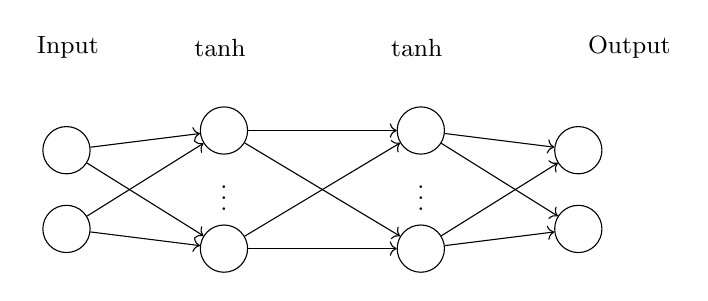
\begin{tikzpicture}[
    node distance=0.5cm,
    neuron/.style={circle, draw, minimum size=0.6cm},
    layer label/.style={font=\small, anchor=west},
    every node/.append style={font=\small}
  ]

  % Input Layer (2 units)
  \node[layer label] at (-.5, 0.3) {Input};
  \foreach \i in {1,2} {
    \node[neuron] (i\i) at (0, -\i) {};
  }

  % Hidden Layer 1 (8 units, condensed)
  \node[layer label] at (1.5, 0.3) {$\tanh$};
  \foreach \i/\y in {1/0.75,3/2.25} {
    \node[neuron] (h1\i) at (2, -\y) {};
  }
  \node at (2, -1.5) {\vdots};

  % Hidden Layer 2 (16 units, condensed)
  \node[layer label] at (4., 0.3) {$\tanh$};
  \foreach \i/\y in {1/0.75,3/2.25} {
    \node[neuron] (h2\i) at (4.5, -\y) {};
  }
  \node at (4.5, -1.5) {\vdots};

  % Output Layer (2 units)
  \node[layer label] at (6.5, 0.3) {Output};
  \foreach \i in {1,2} {
    \node[neuron] (o\i) at (6.5, -\i) {};
  }

  % Connections (sparse for clarity)
  \foreach \i in {1,2} {
    \foreach \j in {1,3} {
      \draw[->] (i\i) -- (h1\j);
    }
  }

  \foreach \i in {1,3} {
    \foreach \j in {1,3} {
      \draw[->] (h1\i) -- (h2\j);
    }
  }

  \foreach \i in {1,3} {
    \foreach \j in {1,2} {
      \draw[->] (h2\i) -- (o\j);
    }
  }

\end{tikzpicture}



\end{document}

